% ==============================================================================
% Kapitel 4: Systematische Literaturübersicht
% ==============================================================================

\section{Systematische Literaturübersicht}
\label{sec:systematische_literaturuebersicht}

Aufbauend auf dem in Kapitel~\ref{sec:forschungsdesign} hergeleiteten methodischen Design beschreibt dieses Kapitel die empirischen und methodischen Ergebnisse der systematischen Literaturübersicht zur Evaluierung und Auswahl von COTS-Software (\textit{Commercial Off-The-Shelf}). Die Beschaffung und Integration kommerzieller Standardsoftwarekomponenten und -pakete stellt eine der weitreichendsten strategischen und architektonischen Weichenstellungen in modernen IT- und Unternehmenslandschaften dar. Eine fehlerhafte oder unzureichend methodisch fundierte Auswahlentscheidung induziert gravierende Folgerisiken: Unvorhergesehene Schnittstellen- und Architekturdiskrepanzen (\textit{Mismatches}), abhaltende Aufwände für nachträgliche Anpassungsprogrammierungen (\textit{Glue-Code}), Performanz- und Sicherheitsengpässe sowie verheerende langfristige Herstellerabhängigkeiten (\textit{Vendor Lock-in}) bedrohen den Erfolg von Softwareprojekten in erheblichem Maße.

Über den 26-jährigen Untersuchungszeitraum von 2000 bis 2026 hat die internationale Forschungsgemeinschaft im Software Engineering und der Wirtschaftsinformatik ein heterogenes Spektrum an methodischen Ansätzen zur Entscheidungsunterstützung hervorgebracht. Diese reichen von frühen qualitativen Bewertungsheuristiken und hierarchischen Paarvergleichsverfahren über nicht-lineare mathematische Portfolio-Optimierungs-modelle und Fuzzy-Entscheidungssysteme bis hin zu modernen kompositionellen, evidenzbasierten und architekturzentrierten Decision Support Systems (DSS).

Ziel dieses Kapitels ist es, diesen verteilten Forschungsstand systematisch aufzubereiten, theoriegeleitet zu strukturieren und in seiner vollen wissenschaftlichen Tiefe zu analysieren. Der Aufbau des Kapitels gliedert sich in drei Hauptabschnitte:
\begin{enumerate}[label=\textbf{\arabic*.}]
  \item \textbf{Abschnitt~\ref{subsec:suchergebnisse_demografie} (Suchergebnisse und Demografie der Literatur):} Dokumentiert den quantitativen Selektionsprozess nach PRISMA 2020, diskutiert das zugehörige Flussdiagramm, analysiert die bibliometrische und institutionelle Demografie der Literatursammlung und legt die Ergebnisse des vierdimensionalen Qualitätsbewertung offen.
  \item \textbf{Abschnitt~\ref{subsec:evolutionaere_abbildung} (Evolutionäre Abbildung der COTS-Auswahlmethoden):} Beantwortet die erste Forschungsfrage durch eine detaillierte historische Rekonstruktion über vier evolutionäre Epochen und würdigt ausnahmslos alle 39 Publikationen in ihren mathematischen, prozeduralen und architektonischen Eigenschaften.
  \item \textbf{Abschnitt~\ref{subsec:morphologische_analyse_ergebnisse} (Morphologische Analyse der COTS-Auswahlmethoden):} Beantwortet die zweite Forschungsfrage anhand der General Morphological Analysis (GMA), analysiert die sechs Parameter des morphologischen Feldes ($N = 2.592$ Konfigurationen), leitet vier methodische Lösungsarchetypen her und analysiert die inhärenten methodischen Kompromisse und praktischen Anwendungsbarrieren.
\end{enumerate}

% ------------------------------------------------------------------------------
% 4.1 Suchergebnisse und Demografie der Literatur
% ------------------------------------------------------------------------------
\subsection{Suchergebnisse und Demografie der Literatur}
\label{subsec:suchergebnisse_demografie}

\subsubsection{Quantitativer Selektionsprozess}
\label{subsubsec:prisma_verlauf}

Die Identifikation und Selektion der Literatursammlung erfolgte unter strikter Einhaltung der PRISMA-2020-Berichtsstandards \parencite{BP42WGEK} sowie des Leitfadenmodells nach \textcite{2NHFUF5N}. Die systematische Suche in den vier wissenschaftlichen Fachdatenbanken erbrachte eine initiale Treffermenge von 761 Datensätzen:
\begin{itemize}[leftmargin=*]
  \item \textbf{IEEE Xplore (IEEE/IET Electronic Library):} 27 Datensätze,
  \item \textbf{ACM Digital Library Premium:} 15 Datensätze,
  \item \textbf{Business Source Premier (EBSCOhost):} 145 Datensätze,
  \item \textbf{Springer Nature eBooks:} 574 Datensätze.
\end{itemize}

Vor Beginn der inhaltlichen Begutachtung wurden die Metadaten in Zotero zusammengeführt. Ein automatisierter und manuell nachgeprüfter Dublettenabgleich identifizierte 16 redundante Datensätze, die eliminiert wurden. Der verbleibende Bereinigungsbestand von 745 Datensätzen wurde dem dreistufigen Screening-Prozess unterzogen.

\begin{figure}[htbp]
  \centering
  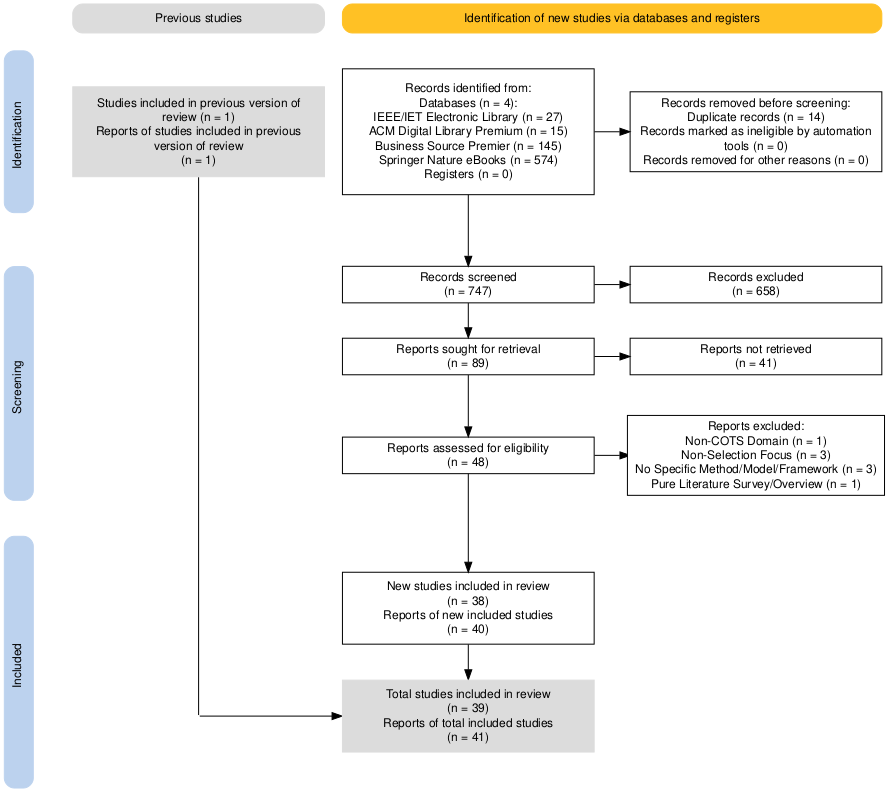
\includegraphics[width=0.82\textwidth]{appendix/prisma_flowchart.png}
  \caption{PRISMA-2020-Flussdiagramm des Such- und Selektionsprozesses \parencite[erstellt über][]{MQ9M8Q7L}}
  \label{fig:prisma_flowchart}
\end{figure}

Wie in Abbildung~\ref{fig:prisma_flowchart} visualisiert, gliederte sich der Selektionsprozess in drei aufeinander aufbauende Stufen:
\begin{enumerate}[label=\textbf{Stufe \arabic*:}, leftmargin=*]
  \item \textbf{Practical Screen 1 (Metadaten-Screening):} Alle 745 Datensätze wurden gegen formale Kriterien geprüft. Ausgeschlossen wurden 597 Publikationen, deren Erscheinungsjahr vor 2000 lag, die nicht in englischer oder deutscher Sprache verfasst waren, reine Vorworte, Konferenz-Inhaltsverzeichnisse oder Editorials darstellten oder keinen fachlichen Bezug zu kommerzieller Standardsoftware aufwiesen. Nach diesem formalen Filter verblieben 148 Publikationen.
  \item \textbf{Practical Screen 2 (Thematisches Relevanz-Screening):} Die 148 Publikationen wurden auf Basis von Titel, Abstract und Schlagwörtern einer Relevanzbewertung auf einer Skala von 1 bis 10 unterzogen. Als Einschlusskriterium galt ein Schwellenwert von $\text{Score} > 7$. Insgesamt wurden 61 Arbeiten exkludiert, die sich primär mit allgemeinen Software-Entwicklungsmethoden im Component-Based Software Engineering (CBSE) ohne Beschaffungs- oder Auswahlsituation befassten, reine Hardware- oder Telekommunikationsinfrastrukturen betrafen oder rein deskriptive Anforderungslisten ohne Entscheidungsmodell diskutierten. 87 Publikationen qualifizierten sich als hochrelevant; unter Berücksichtigung zweier methodischer Grenzfälle wurden 89 Volltexte zur Beschaffung angefordert.
  \item \textbf{Practical Screen 3 (Volltextbeschaffung und Eligibility-Screening):} Von den 89 angeforderten Volltexten konnten über die Hochschullizenzen der DHBW CAS sowie Open-Access-Zugriff 46 Volltexte erfolgreich abgerufen werden. 43 Volltexte waren aufgrund geschlossener fehlender Hochschullizenzen nicht zugänglich (\textit{not retrieved}). Die 46 beschafften Volltexte wurden einer vollständigen inhaltlichen Prüfung gegen die definierten hierarchischer Ausschlusskriterien unterzogen. Acht Volltexte wurden dadurch exkludiert:
  \begin{itemize}[leftmargin=*]
    \item \textit{Ausschlussgrund 1.1 (Non-COTS Domain, $N = 1$):} Der Fokus lag ausschließlich auf der physischen Hardware- und Netzwerkauswahl.
    \item \textit{Ausschlussgrund 1.2 (Non-Selection Focus, $N = 3$):} Die Arbeiten behandelten keine Auswahlsituationen.
    \item \textit{Ausschlussgrund 2.1 (No Specific Method/Model/Framework, $N = 3$):} Reine konzeptionelle Diskussionen oder abstrakte Management-Empfehlungen ohne operationalisiertes mathematisches oder prozedurales Bewertungsmodell.
    \item \textit{Ausschlussgrund 2.2 (Pure Literature Survey / Overview, $N = 1$):} Sekundäre Übersichtsarbeit ohne eigenständigen methodischen Beitrag.
  \end{itemize}
\end{enumerate}

Eine zentrale Publikation wurde aus der Proposal-Recherche integriert, bei der es sich um das COTS-ESF Framework von \textcite{WZM7DUBY} handelt. Die finale Literatursammlung umfasst somit exakt 39 Publikationen (\textit{Reports}), welche 38 unabhängige Primärstudien (\textit{Studies}) repräsentieren, da die Publikationen von \textcite{ZQMG69VT} und \textcite{MZ8JHDYA} als zusammengehöriges Forschungscluster bewertet werden.

\subsubsection{Demografische und bibliometrische Struktur der Literatursammlung}
\label{subsubsec:demografie_korpus}

Die bibliometrische Analyse der Literatursammlung über den Zeitraum 2000 bis 2026 zeigt eine kontinuierliche wissenschaftliche Befassung mit der COTS-Auswahlproblematik. Tabelle~\ref{tab:demografie_qa_uebersicht} fasst die demografischen Kernkennzahlen, Publikationskanäle und Quality-Appraisal-Ergebnisse zusammen.

\begin{table}[htbp]
  \centering
  \small
  \caption{Aggregierte demografische Kennzahlen und Qualitätsverteilung ($N = 39$)}
  \label{tab:demografie_qa_uebersicht}
  \begin{tabularx}{\textwidth}{>{\bfseries\raggedright\arraybackslash}p{3.2cm}>{\raggedright\arraybackslash}Xcc}
    \toprule
    Dimension & Primäre Kategorien im Korpus & Studien ($N$) & Anteil (\%) \\
    \midrule
    Publikationszeitraum & 2000--2009 / 2010--2019 / 2020--2026 & 16 / 13 / 10 & 41,0\,\% / 33,3\,\% / 25,6\,\% \\
    Publikationsorgan & Fachzeitschriften / Konferenzen / Monographien & 21 / 14 / 4 & 53,8\,\% / 35,9\,\% / 10,3\,\% \\
    Evidenzklasse (QA) & Hohe Evidenz (6--8 P.) / Mittlere (3--5 P.) / Niedrig & 36 / 2 / 1 & 92,3\,\% / 5,1\,\% / 2,6\,\% \\
    \midrule
    \multicolumn{4}{p{\dimexpr\textwidth-2\tabcolsep\relax}}{\textbf{Mittelwerte:} QA1: 1,87 \quad QA2: 1,87 \quad QA3: 1,56 \quad QA4: 1,56 \quad \textbf{Gesamt-Mittelwert: 6,87 / 8,00 P.}} \\
    \bottomrule
  \end{tabularx}
\end{table}

In der Dekade 2000--2009 erschienen 16 Publikationen (41,0\,\%). Diese Pionierphase war geprägt von der Etablierung erster Outranking- und AHP-Modelle sowie dem Entwurf dedizierter Software-Werkzeuge. In der zweiten Dekade (2010--2019) wurden 13 Publikationen (33,3\,\%) publiziert, in denen die mathematische Optimierung, nicht-lineare Programmierung und Fuzzy-MCDA-Verfahren dominierten. Die jüngste Phase (2020--2026) steuert 10 Publikationen (25,6\,\%) bei, die sich auf kompositionelle Datenanalysen, Evidential Reasoning und großangelegte Meta-Synthesen konzentrieren.

Hinsichtlich der Publikationsorgane stellen internationale Fachzeitschriften mit 53,8\,\% ($N = 21$) den Hauptanteil dar. Darunter befinden sich renommierte Journals wie \textit{Information Systems Frontiers} \parencite{FCYW9EWJ}, \textit{Information and Software Technology} \parencite{8VHUMEKY}, \textit{Applied Intelligence} \parencite{B7ZTQCZZ, JX4RDRDU}, \textit{Software Quality Journal} \parencite{M3B2D3GD}, \textit{Requirements Engineering} \parencite{DAU8NSK8}, \textit{Annals of Operations Research} \parencite{YVWGHAWQ} und \textit{Complex \& Intelligent Systems} \parencite{UFCEV52H}. Konferenzbeiträge umfassen 35,9\,\% ($N = 14$), unter anderem von der \textit{IEEE Asia-Pacific Services Computing Conference} \parencite{MZ8JHDYA} und der \textit{International Conference on Commercial-off-the-Shelf (COTS)-Based Software Systems (ICCBSS)} \parencite{6RNULWVY}. Hinzu kommen vier wegweisende Dissertationen \parencite{ 9F79VAAB, WBGP3ETU, WZM7DUBY, RRU375GB}.

Geografisch und institutionell lassen sich vier globale Forschungsschwerpunkte identifizieren:
\begin{itemize}[leftmargin=*]
  \item \textbf{Nordamerika:} Die University of Calgary (Kanada) formierte mit den Arbeiten von \textcite{CZZ6XQZJ} und \textcite{9F79VAAB} eine führende Gruppe für Multi-Stakeholder-Verhandlungen und architekturzentriertes Mismatch-Handling. In den USA erforschten \textcite{QDUNCXFC} am NASA Langley Research Center sowie University of Virginia probabilistische Bayes-Netze für sicherheitskritische Raumfahrtsysteme, während \textcite{CI86GRRG} und \textcite{6RNULWVY} an der University of Texas at Dallas modellgetriebene Anforderungs- und Fuzzy-Auswahlverfahren entwickelten.
      \item \textbf{Mitteleuropa:} In Österreich etablierten \textcite{ZQMG69VT} und \textcite{MZ8JHDYA} am Secure Business Austria und der Universität Wien interaktive Mehrzieloptimierungs- und Pareto-DSS-Engines. An der TU Wien konzipierten \textcite{8VHUMEKY} das Plato-System zur automatisierten Benchmark-Evaluation. In Deutschland legten \textcite{WBGP3ETU} an der Universität Augsburg und \textcite{RRU375GB} an der Universität Bamberg umfassende Arbeiten zu Make-or-Buy-Strategien und IoT-Plattformen vor.
  \item \textbf{Südeuropa und Skandinavien:} An der Universitat Politècnica de Catalunya prägte \textcite{TLB687YL} zielorientierte Anforderungsmodelle. An der Universität Paris-Dauphine entwickelten \textcite{LZQJ6M4X} und \textcite{M3B2D3GD} frühe Outranking-Verfahren auf Basis der ISO 9126. Am Politecnico di Milano untersuchten \textcite{DAU8NSK8} empirische AHP-Modelle. In Schweden trieben \textcite{JT5X3FIG} an der Blekinge Institute of Technology und \textcite{UK2X9C4W} an der Universität Lund strategische Sourcing-Taxonomien und kompositionelle Datenanalysen voran.
  \item \textbf{Asien (insbesondere Indien):} Eine außergewöhnlich dichte Serie mathematischer Optimierungs- und Fuzzy-MCDA-Arbeiten entstand an der University of Delhi und der Netaji Subhas University of Technology \parencite{VUVLUN85, 6YJHIVHG, P9SATBH5, B7ZTQCZZ, JX4RDRDU, YVWGHAWQ, 8KF4HAZS}, ergänzt durch Arbeiten der Amity University \parencite{DFASRUVC}, des NITIE Mumbai \parencite{U4E7VXQU} und der PDEU Gujarat \parencite{5BBYQCJB}.
\end{itemize}

\subsubsection{Ergebnisse der Qualitätsbewertung}
\label{subsubsec:qa_ergebnisse}

Die vierdimensionale Qualitätsbewertung bescheinigt der Literatursammlung eine exzellente wissenschaftliche Belastbarkeit. Mit einem Gesamtmittelwert von \textbf{6,87 von 8,00 Punkten} erreichen 36 der 39 Publikationen (92,3\,\%) die höchste Evidenzklasse. Zwei Publikationen (5,1\,\%) fallen in die mittlere Evidenzklasse, während lediglich ein früher konzeptioneller Entwurf (2,6\,\%) der niedrigsten Evidenzklasse zugeordnet wurde.

Die Detailanalyse der Einzeldimensionen (jeweils normiert auf 0 bis 2 Punkte) zeigt folgende Ausprägungen:
\begin{itemize}[leftmargin=*]
  \item \textbf{QA1 (Methodische Transparenz und Formalisierung -- Mittelwert: 1,87):} 34 Publikationen erzielten die Maximalpunktzahl von 2 Punkten. Die mathematischen und algorithmischen Modelle -- von AHP-Supermatrizen über nicht-lineare ganzzahlige Optimierungsgleichungen bis hin zu Dempster-Shafer-Evidenzregeln -- sind formelhaft lückenlos und reproduzierbar spezifiziert.
  \item \textbf{QA2 (Transparenz des Kriterienkatalogs -- Mittelwert: 1,87):} Ebenfalls 34 Publikationen legen vollständig strukturierte, hierarchisch gegliederte Kriterienkataloge offen. Lediglich fünf Publikationen beschränken sich auf unvollständige Beispiellisten.
  \item \textbf{QA3 (Empirische Validierung und Evidenzniveau -- Mittelwert: 1,56):} 22 Publikationen (56,4\,\%) weisen eine reale empirische Validierung anhand von Industrie-Fallstudien, Praktiker-Umfragen oder kontrollierten Experimenten auf. 14 Publikationen demonstrieren ihre Algorithmen an synthetischen numerischen Benchmarks, während drei Publikationen rein theoretisch verbleiben.
  \item \textbf{QA4 (Kritische Reflexion von Grenzen und Kontextfaktoren -- Mittelwert: 1,56):} 22 Publikationen diskutieren Limitationen, kognitiven Aufwand, Rechenkomplexität und Validitätsrisiken tiefgründig. 17 Publikationen begnügen sich mit kurzen methodischen Anmerkungen.
\end{itemize}

% ------------------------------------------------------------------------------
% 4.2 Evolutionäre Abbildung der COTS-Auswahlmethoden
% ------------------------------------------------------------------------------
\subsection{Evolutionäre Abbildung der COTS-Auswahlmethoden}
\label{subsec:evolutionaere_abbildung}

Zur Beantwortung von Forschungsfrage 1 rekonstruiert dieser Abschnitt die historische Entwicklungslinie anhand von vier chronologischen Epochen. Alle 39 Publikationen werden nachfolgend in ihren mathematischen, architektonischen und prozeduralen Beiträgen detailliert analysiert und gewürdigt. Tabelle~\ref{tab:evolutionaere_epochen} bietet eine systematische Übersicht über die Epochen, Leitprofile und Zeiträume (die ausführliche Epochenmatrix mit allen Übergangstreibern ist in Anhang~D, Tabelle~\ref{tab:anhang_epochen_matrix}, dokumentiert).

\begin{table}[htbp]
  \centering
  \small
  \caption{Evolutionäre Epochen der COTS-Softwareauswahl (2000--2026)}
  \label{tab:evolutionaere_epochen}
  \begin{tabularx}{\textwidth}{>{\bfseries\raggedright\arraybackslash}p{2.6cm}>{\raggedright\arraybackslash}p{2.8cm}>{\raggedright\arraybackslash}Xcc}
    \toprule
    Epoche & Zeitraum & Zentrales methodisches Paradigma & Studien ($N$) & Anteil \\
    \midrule
    Epoche 1 & 2000 bis 2005 & Outranking- \& AHP-Modelle (ISO 9126) & 10 & 25,6\,\% \\
    Epoche 2 & 2006 bis 2011 & Architektur, Mismatch-Handling \& DSS & 11 & 28,2\,\% \\
    Epoche 3 & 2012 bis 2019 & Mathematische Optimierung \& Fuzzy-MCDA & 12 & 30,8\,\% \\
    Epoche 4 & 2020 bis 2026 & CoDa, Evidential Reasoning \& Synthesen & 6 & 15,4\,\% \\
    \bottomrule
  \end{tabularx}
\end{table}

\subsubsection{Epoche 1 (2000 bis 2005): Grundlegende Outranking- und frühe Mehrkriterien-Frameworks}
\label{subsubsec:epoche1}

Die erste Epoche (2000 bis 2005) markiert den Übergang von rein informellen, intuitiven Beschaffungsentscheidungen zu formalisierten mathematischen und prozeduralen Bewertungsverfahren. Angesichts explodierender Fehlerraten bei der Einführung unternehmensweiter Softwaresysteme bestand das primäre Ziel darin, die Auswahlentscheidung transparent, objektiv und kriteriengeleitet zu gestalten.

Den Beginn markieren Arbeiten aus dem Bereich der europäischen Outranking-Methode. \textcite{LZQJ6M4X} demonstrierten anhand eines realen Beschaffungsprojekts bei Telecom Italia den Einsatz von ELECTRE-TRI zur Vorfilterung und Klassifikation kommerzieller Angebote im Rahmen öffentlicher Ausschreibungen (\textit{Calls for Tenders}). Ihr Ansatz nutzte Konkordanz- und Diskordanzschwellen, um unzureichende Softwarekandidaten über Veto-Regeln auszusortieren. Der fundamentale Vorteil dieses Outranking-Ansatzes lag in seiner Nicht-Kompensatorik: Gravierende Schwächen in funktionalen Kernanforderungen durften nicht durch hervorragende Werte in Nebenkriterien kompensiert werden. Aufbauend auf dieser Arbeit stellten \textcite{M3B2D3GD} die erste formale Verbindung zwischen Outranking-Relationen und dem internationalen Qualitätsstandard ISO/IEC 9126 her. Sie wiesen mathematisch nach, dass naive additive Aggregationen (wie das klassische gewichtete Punktwertmodell WSM) auf ordinalen Qualitätsmetriken unzulässig sind und führten Präferenz- sowie Indifferenzschwellen zur Vermeidung von Fehlinterpretationen ein.

Parallel dazu etablierten sich hierarchische und netzwerkartige Verfahren. \textcite{DAU8NSK8} operationalisierten den Analytic Hierarchy Process (AHP) auf Basis der ISO/IEC 9126 und validierten das Modell empirisch an einer Stichprobe von 42 kommerziellen CRM-Paketen. Sie zeigten, dass AHP Entscheidungsträgern erlaubt, funktionale Eignung, technische Qualität und Kostenstrukturen strukturiert gegeneinander abzuwägen. Da hierarchische Bäume jedoch Wechselwirkungen zwischen Kriterien vernachlässigen, führten \textcite{FCYW9EWJ} den Analytic Network Process (ANP) in die COTS-Evaluation ein. Mittels Supermatrizen bildeten sie wechselseitige Abhängigkeiten zwischen betriebswirtschaftlichen Kernprozessen, bestehender Legacy-Infrastruktur und Softwareattributen formelhaft ab.

Für hochgradig sicherheitskritische Anwendungsdomänen reichten deterministische Bewertungsbäume nicht aus. \textcite{QDUNCXFC} entwickelten für das \textit{Cockpit Avionics Upgrade} (CAU) des NASA Space Shuttles ein probabilistisches Entscheidungsmodell auf Basis von Bayesian Belief Networks (BBN). Durch die Hinterlegung bedingter Wahrscheinlichkeitstabellen (\textit{Conditional Probability Tables}, CPTs) gelang es, extreme Unsicherheiten hinsichtlich Echtzeitfähigkeit, Speicherzuverlässigkeit und Flugzertifizierung kommerzieller Echtzeitbetriebssysteme (RTOS) mathematisch präzise zu modellieren.

Gleichzeitig entstanden erste hybride und anforderungszentrierte Ansätze. \textcite{CI86GRRG} integrierten Fuzzy-Regelsysteme und Adaptive Neuro-Fuzzy Inference Systems (ANFIS), um Unschärfen in Dienstgütemetriken (QoS) von COTS-Komponenten auszugleichen. \textcite{TLB687YL} konzipierte einen leichtgewichtigen zielorientierten Modellierungsansatz auf Basis des $i^*$-Strategic Dependency Models, der relationale Abhängigkeiten zwischen Organisationszielen (\textit{Strategic Dependency}) und Softwarefähigkeiten (\textit{Strategic Rationale}) analysierte. \textcite{CZZ6XQZJ} legten mit NeMo-CoSe ein Verhandlungsmodell vor, das spieltheoretische Win-Win-Konditionen zwischen heterogenen Stakeholder-Gruppen bei der Komponentenauswahl formalisierte.

\subsubsection{Epoche 2 (2006 bis 2011): Architekturintegration, Mismatch-Behandlung und dedizierte DSS-Engines}
\label{subsubsec:epoche2}

Die zweite Epoche (2006 bis 2011) brachte eine entscheidende architektonische Wende hervor. Die wissenschaftliche Gemeinschaft erkannte, dass Standardsoftwarekomponenten isoliert selten perfekt in bestehende Systemlandschaften passen. Der Forschungsschwerpunkt verlagerte sich daher von der reinen Blackbox-Bewertung hin zur aktiven Mismatch-Erkennung, architektonischen Verträglichkeitsprüfung und der Entwicklung eigenständiger Decision Support Systems (DSS).

\textcite{8XNYS4M9} operationalisierten funktionale Diskrepanzen, indem sie auf Basis von ISO/IEC 9126-2 ein formales Messmodell für funktionale Eignung entwickelten. Dieses differenzierte zwischen funktionaler Vollständigkeit (\textit{Completeness}), Adäquatheit (\textit{Adequacy}) und funktionalem Überhang (\textit{Excess}) und balancierte diese Metriken über AHP-Stakeholdergewichte im E-Payment-Kontext. \textcite{6RNULWVY} automatisierten den Anforderungsabgleich im CARE-Framework (\textit{Component-Aware Requirements Engineering}), indem sie syntaktische Baum-Editierdistanzen mit semantischen WordNet-Ontologien kombinierten, um funktionale \enquote{Near-Miss}-Kandidaten über Softgoal Interdependency Graphs (SIG) algorithmisch zu identifizieren. \textcite{U5JPV4SF} präsentierte eine Hybridisierung, die ANP zur Modellierung von Kriterieninterdependenzen mit einem modifizierten TOPSIS-Algorithmus vereinte, um Workflow-Management-Systeme anhand euklidischer Distanzen zu idealen Referenzpunkten zu bewerten.

Einen Meilenstein setzte die Dissertation von \textcite{9F79VAAB}, der das MiHOS-Framework (\textit{Mismatch Handling aware COTS Selection}) schuf. Mohamed systematisierte funktionale, architektonische und nicht-funktionale Inkompatibilitäten in einer fundierten Taxonomie und integrierte die mathematische Planung von Anpassungsmaßnahmen (z.\,B. Glue-Code, Wrapper-Synthese) direkt in das Auswahl-DSS, begleitet durch die neuartige Sensitivitätsanalyse IDS-SA.

Parallel dazu revolutionierten \textcite{ZQMG69VT} und \textcite{MZ8JHDYA} die multikriterielle Entscheidungsfindung: Anstatt Entscheidungsträger zu zwingen, Kriteriengewichte \textit{a priori} festzulegen -- was bei unvollständiger Marktkenntnis regelmäßig zu Fehlentscheidungen führt -- formulierten sie das Auswahlproblem als multikriterielle 0-1-Ganzzahlprogrammierung. In ihrem interaktiven DSS-Werkzeug Atana/Odin erkunden Entscheidungsträger interaktiv die Pareto-optimale Lösungsfront. Dadurch wird kognitive Überlastung vermieden und Portfolio-Kombinationen werden ohne a-priori-Gewichtsverzerrungen identifiziert, wie die Validierung im österreichischen Sozialversicherungssektor (MediCorp-Fallstudie) belegte.

Weitere spezialisierte DSS-Artefakte entstanden in dieser Phase: \textcite{8VHUMEKY} entwickelten das Plato-DSS für digitale Langzeitarchivierung, das subjektive Experteneinschätzungen durch vollautomatisierte empirische Benchmark-Messreihen und objektive Nutzenbäume ersetzte. \textcite{VUVLUN85} formulierten ein nicht-lineares 0-1-Optimierungsmodell zur Komponentenauswahl unter fehlertoleranten \textit{Recovery Block} (RB) Architekturen, das Zuverlässigkeit, Kosten und Ausführungszeit simultan optimierte. \textcite{WBGP3ETU} strukturierte die strategische Make-or-Buy-Entscheidung architektonisch, während \textcite{U4E7VXQU} mit HKBS ein wissensbasiertes System schufen, das regelbasierte Vorabfilterung, fallbasiertes Schließen (\textit{CBRank}) und AHP vereinte.

\subsubsection{Epoche 3 (2012 bis 2019): Mathematische Optimierung und Ausbreitung von Fuzzy-MCDA}
\label{subsubsec:epoche3}

Die dritte Epoche (2012--2019) war durch eine massive Mathematisierung und die Ausbreitung der Fuzzy-Set-Theorie gekennzeichnet. Die Wissenschaftliche Gemeinschaft reagierte damit auf die Erkenntnis, dass Expertenurteile bei komplexen Softwarebeschaffungen naturgemäß vage, linguistisch geprägt und mit erkenntnistheoretischer Unsicherheit behaftet sind.

\textcite{6YJHIVHG} formulierten ein interaktives Fuzzy-Mathematisches Programmierungsmodell (FMP), das ISO-9126-Qualitätsmetriken in eine simultane Optimierung von Kosten, Zuverlässigkeit, Lieferzeit und Ausführungszeit modularer Systeme einbettete. \textcite{W8P543Y2} erweiterten MCDM-Systeme für Cloud-basierte SaaS-ERP-Systeme um dynamische QoS-Messungen und Social-Network-Reputationsbewertungen. \textcite{VRTXHQI7} entwickelten ein hybrides Fuzzy-MCDA-Modell für CAD/CAM-Software, das die relative Nähe zur idealen Lösung via Fuzzy-TOPSIS mit den nicht-kompensatorischen Veto-Schwellen von Fuzzy-ELECTRE kombinierte.

\textcite{WZM7DUBY} entwickelte in seiner Dissertation das COTS-ESF-Framework, das AHP-Gewichtungen mathematisch mit quantitativer Gap-Analyse verknüpfte, um Anpassungsaufwände und Schnittstellenrisiken vor der Kaufentscheidung formelhaft zu quantifizieren. \textcite{LYMHTPXS} operationalisierten die neu verabschiedete Qualitätsnorm ISO/IEC 25010 für ein gewichtetes Attribut-Scoring proprietärer und quelloffener BPMS-Werkzeuge.

Eine Serie mathematisch hochgradig anspruchsvoller Arbeiten stammte von der Forschergruppe um Gupta, Mehlawat, Jha und Verma: \textcite{P9SATBH5} modellierten die Komponentenauswahl unter einem fehlertoleranten \textit{Consensus Recovery Block} (CRB) Schema mittels Fuzzy-Nichtlinearer Optimierung in LINGO. \textcite{B7ZTQCZZ} kombinierten Fuzzy-TOPSIS mit kompensatorischen Credibility-Chance-Constrained-Modellen, während \textcite{JX4RDRDU} ein multikriterielles kredibilistisches 0-1-Programmierungsmodell vorlegten, das Erwartungswert- und Zufallsparameter unter Fuzzy-Glaubwürdigkeitsmaßen simultan steuerte.

Ergänzt wurde diese Phase durch hierarchische Wiederverwendungsmodelle von \textcite{DFASRUVC}, das strategische GRADE-Sourcing-Framework von \textcite{JT5X3FIG}, die methodische Triangulation aus Delphi-Filterung, Fuzzy-AHP und PROMETHEE-II-Outranking-Flüssen von \textcite{NZJEEPAC} sowie die Usability-fokussierte AHP-VIKOR-Kompromissrangbildung von \textcite{QNWK8SAP}.

\subsubsection{Epoche 4 (2020 bis 2026): Kompositionelle Daten, Evidential Reasoning und Meta-Analysen}
\label{subsubsec:epoche4}

Die jüngste Epoche (2020 bis 2026) zeichnet sich durch methodische Reifung, die Beseitigung struktureller mathematischer Verzerrungen klassischer Verfahren sowie breit angelegte empirische und methodische Meta-Analysen aus.

Einen herausragenden methodenkritischen Beitrag leisteten \textcite{UK2X9C4W}: Sie wiesen mathematisch nach, dass traditionelle Punkteverteilungsverfahren wie das Cumulative Voting (\$100-Test) aufgrund der konstanten Summenrestriktion im Simplex-Raum massiven statistischen Scheinkorrelationen unterliegen. Durch die Einführung der \textit{Compositional Data Analysis} (CoDa) mit Centered Log Ratio (CLR) Transformationen etablierten sie ein verzerrungsfreies statistisches Fundament zur Priorisierung von ISO/IEC-25010-Qualitätsattributen, validiert an 157 Software-Praktikern.

\textcite{5BBYQCJB} validierten empirisch ein Fuzzy-AHP-Modell mit Dreiecks-Fuzzy-Zahlen zur ERP-Auswahl in Industrieunternehmen. \textcite{UFCEV52H} führten das Konzept der \textit{Fuzzy Intra-Coupling Density} (Fuzzy-ICD) in ein nicht-lineares 0-1-Ganzzahlmodell ein, um modulare Kopplungen und Kohäsionen in Build-or-Buy-Architekturen simultan mit Kosten und Zuverlässigkeit zu optimieren.

Einen Höhepunkt der Evidenzkonsolidierung bildet die 588-seitige DSR-Monographie von \textcite{RRU375GB}, die in einer Meta-Analyse von 139 COTS-Publikationen den State-of-the-Art systematisierte und einen ganzheitlichen Kriterienkatalog sowie eine Referenzarchitektur für IoT-Softwareplattformen entwickelte. \textcite{FVINCQ89} präsentierte den FMDBA-Ansatz (\textit{Fuzzy Modified Distance-Based Approach}), der subjektive Expertengewichte mit objektiver Fuzzy-Entropie fusionierte. \textcite{YVWGHAWQ} verknüpften die Effizienzgrenzen der Data Envelopment Analysis (DEA) mit evolutionären NSGA-II-Algorithmen zur Komponentenauswahl unter optimaler Redundanz. \textcite{8KF4HAZS} etablierten ein Zwei-Phasen-Framework aus Fuzzy-TOPSIS und interaktiver Optimierung für Multi-Applikations-Suiten.

Einen wegweisenden Schritt zur Behandlung erkenntnistheoretischer Unvollständigkeit vollzog \textcite{LNQHES84} durch den Einsatz des Evidential Reasoning (ER) auf Basis der Dempster-Shafer-Theorie. Dieses Modell erlaubt es, unvollständige Anbieterauskünfte und konfligierende Gutachterbewertungen über Glaubensverteilungen (\textit{Belief Distributions}) und Nichtwissensgrade mathematisch exakt abzubilden. Schließlich lieferten \textcite{LPC92LAP} eine kritische Meta-Analyse über 41 Arbeiten zum Einsatz von MCDM im Software Engineering, in der sie Phänomene der Rangumkehr (\textit{Rank Reversal}) und kognitive Überlastungen beleuchteten.

% ------------------------------------------------------------------------------
% 4.3 Morphologische Analyse der COTS-Auswahlmethoden
% ------------------------------------------------------------------------------
\subsection{Morphologische Analyse der COTS-Auswahlmethoden}
\label{subsec:morphologische_analyse_ergebnisse}

Zur Beantwortung von Forschungsfrage 2 wird die in Abschnitt~\ref{subsec:morphologische_analyse_methodik} hergeleitete General Morphological Analysis (GMA) nach Zwicky und Ritchey \parencite[S.~81 bis 91]{Z6N6V5L9} empirisch auf die Literatursammlung angewendet.

\subsubsection{Induktive Konstruktion des morphologischen Feldes}
\label{subsubsec:feldkonstruktion}

Die sechs Schlüsselparameter ($P_1 \dots P_6$) und ihre diskreten Ausprägungen wurden induktiv und theoriegeleitet aus den Merkmalen der 17-spaltigen Datenextraktionsmatrix (Abschnitt~\ref{subsec:qualitaetsbewertung_datenextraktion}) abgeleitet. Sie erfüllen die formalen Bedingungen der Parameter-Orthogonalität (wechselseitiger Ausschluss) und kollektiven Erschöpfung \parencite[vgl.][S.~82 bis 83]{Z6N6V5L9}:
\begin{enumerate}[label=\textbf{\arabic*.}, leftmargin=*]
  \item \textbf{$P_1$ (Mathematisches Entscheidungs- und Gewichtungsmodell):} Operationalisiert das fundamentale mathematische Paradigma aus den Extraktionsfeldern \\ \texttt{Mathematical\_Decision\_Model} und \texttt{Primary\_Methodological\_Approach}. Es umfasst $|P_1| = 6$ disjunkte Ausprägungen: klassische MCDA ($v_{1.1}$), Outranking ($v_{1.2}$), mathematische Optimierung ($v_{1.3}$), Fuzzy-MCDA/OR ($v_{1.4}$), probabilistische/wissensbasierte KI ($v_{1.5}$) und rein qualitative/zielorientierte Modelle ($v_{1.6}$).
  \item \textbf{$P_2$ (Entscheidungsunterstützungs-Automatisierung):} Erfasst den werkzeugtechnischen Reifegrad aus dem Feld \texttt{Decision\_Support\_Automation} mit $|P_2| = 3$ Ausprägungen: manuelle Leitfäden ($v_{2.1}$), Solver/Skripte/Tabellenkalkulationen ($v_{2.2}$) und vollwertige interaktive Decision Support Systems mit GUI ($v_{2.3}$).
  \item \textbf{$P_3$ (Mismatch- und Inkompatibilitätsbehandlung):} Systematisiert die architektonische Integrationsfähigkeit aus den Feldern \texttt{Mismatch\_Handling} und \\ \texttt{Mismatch\_Handling\_Phase} mit $|P_3| = 4$ Ausprägungen: keine Behandlung ($v_{3.1}$), Vorabfilterung ($v_{3.2}$), mathematische Nebenbedingungen ($v_{3.3}$) und post-selektive Adaptationsplanung inklusive Schnittstellen-/Wrapper-Kosten ($v_{3.4}$).
  \item \textbf{$P_4$ (Unsicherheits- und Unschärfemodellierung):} Klassifiziert den mathematischen Umgang mit epistemischer und stochastischer Vagheit aus dem Feld \\ \texttt{Uncertainty\_Handling} mit $|P_4| = 4$ Ausprägungen: deterministische Punktwerte ($v_{4.1}$), Fuzzy-Set-Theorie ($v_{4.2}$), Sensitivitäts-/Intervallanalysen inklusive CoDa ($v_{4.3}$) und probabilistische Bayes-/Evidenztheorie ($v_{4.4}$).
  \item \textbf{$P_5$ (Umfang des Kriterienkatalogs):} Bildet die inhaltliche Bewertungsbreite aus dem Feld \texttt{Covered\_Criteria\_Types} mit $|P_5| = 3$ Ausprägungen ab: rein funktionale Eignung ($v_{5.1}$), Softwarequalität und Performance ($v_{5.2}$) sowie ganzheitlich-mehrdimensionale Kriterienbäume ($v_{5.3}$).
  \item \textbf{$P_6$ (Kriterien-Standardisierung und Wiederverwendbarkeit):} Erfasst den Grad der normativen Verankerung aus dem Feld \texttt{Criteria\_Catalog\_Structure} mit $|P_6| = 3$ Ausprägungen: ad-hoc generiert ($v_{6.1}$), standardbasiert nach ISO/IEC 9126 bzw. ISO/IEC 25010 ($v_{6.2}$) und wiederverwendbare Ontologien bzw. Wissensbasen ($v_{6.3}$).
\end{enumerate}

Das kartesische Produkt der Parameterdomänen spannt einen theoretischen Gesamtraum von
\begin{equation}
  N = \prod_{i=1}^{6} |P_i| = 6 \times 3 \times 4 \times 4 \times 3 \times 3 = 2.592 \text{ Konfigurationen} \notag
\end{equation}
auf. Tabelle~\ref{tab:morphologisches_feld} fasst die sechs Dimensionen des morphologischen Feldes zusammen (das vollständige morphologische Feld mit allen 25 diskreten Ausprägungen und Definitionen ist in Anhang~F, Tabelle~\ref{tab:anhang_morphologisches_feld}, dokumentiert).

\begin{table}[htbp]
  \centering
  \small
  \caption{Übersicht der sechs morphologischen Dimensionen ($N = 2.592$ Konfigurationen)}
  \label{tab:morphologisches_feld}
  \begin{tabularx}{\textwidth}{cl>{\raggedright\arraybackslash}Xcc}
    \toprule
    \textbf{ID} & \textbf{Morphologischer Parameter} & \textbf{Dominante Ausprägung im Korpus} & \textbf{$N$} & \textbf{Anteil} \\
    \midrule
    $P_1$ & Mathematisches Entscheidungsmodell & Fuzzy-MCDA \& Fuzzy-OR ($v_{1.4}$) & 11 & 28,2\,\% \\
    $P_2$ & Automatisierungsgrad & Skripte, Tabellen \& Solver ($v_{2.2}$) & 21 & 53,8\,\% \\
    $P_3$ & Mismatch-Behandlung & Vorabfilterung ($v_{3.2}$) / Nebenbedingungen ($v_{3.3}$) & je 15 & je 38,5\,\% \\
    $P_4$ & Unsicherheitsmodellierung & Deterministisch ($v_{4.1}$) / Fuzzy-Sets ($v_{4.2}$) & 16 / 13 & 41,0\,\% / 33,3\,\% \\
    $P_5$ & Kriterienkatalog-Umfang & Ganzheitlich mehrdimensional ($v_{5.3}$) & 22 & 56,4\,\% \\
    $P_6$ & Kriterien-Standardisierung & Ad-hoc projektspezifisch generiert ($v_{6.1}$) & 19 & 48,7\,\% \\
    \bottomrule
  \end{tabularx}
\end{table}

\subsubsection{Parameteranalyse des morphologischen Feldes}
\label{subsubsec:parameteranalyse}

Die relative Häufigkeitsverteilung über alle sechs Parameter gliedert sich wie folgt:
\begin{itemize}[leftmargin=*]
  \item \textbf{$P_1$ (Mathematisches Entscheidungs- und Gewichtungsmodell):} Das Feld wird von Fuzzy-MCDA- und Fuzzy-OR-Modellen dominiert ($v_{1.4}$: 28,2\,\%, $N = 11$), gefolgt von klassischen deterministischen MCDA-Ansätzen ($v_{1.1}$: 23,1\,\%, $N = 9$). Qualitative und prozessorientierte Modelle umfassen 17,9\,\% ($v_{1.6}$, $N = 7$), während probabilistische, evidenzbasierte und wissensbasierte Systeme 15,4\,\% stellen ($v_{1.5}$, $N = 6$). Mathematische Optimierungsmodelle ($v_{1.3}$: 10,3\,\%, $N = 4$) und reine Outranking-Verfahren ($v_{1.2}$: 5,1\,\%, $N = 2$) bilden spezialisierte Nischen.
  \item \textbf{$P_2$ (Automatisierungsgrad der Entscheidungsunterstützung):} Mehr als die Hälfte aller Publikationen ($v_{2.2}$: 53,8\,\%, $N = 21$) stützt sich auf mathematische Skripte, Tabellenkalkulationen oder kommerzielle OR-Solver (z.\,B. LINGO, MATLAB). 28,2\,\% ($v_{2.3}$, $N = 11$) implementieren vollwertige interaktive Decision Support Systems mit eigener GUI. 17,9\,\% ($v_{2.1}$, $N = 7$) verbleiben auf Ebene manueller prozeduraler Richtlinien.
  \item \textbf{$P_3$ (Mismatch- und Inkompatibilitätsbehandlung):} Jeweils 38,5\,\% ($N = 15$) nutzen Vorabfilterung ($v_{3.2}$) oder mathematische Nebenbedingungen ($v_{3.3}$). Dagegen adressieren lediglich 10,3\,\% ($v_{3.4}$, $N = 4$) die fundamentale post-selektive Adaptationsplanung (Glue-Code, Gap Analysis). 12,8\,\% ($v_{3.1}$, $N = 5$) ignorieren Mismatches vollständig.
  \item \textbf{$P_4$ (Unsicherheits- und Unschärfemodellierung):} 41,0\,\% ($v_{4.1}$, $N = 16$) arbeiten rein deterministisch mit Einzelwerten. 33,3\,\% ($v_{4.2}$, $N = 13$) modellieren Unschärfe über Fuzzy-Zahlen. Sensitivitätsanalysen und CoDa-Log-Ratios stellen 17,9\,\% ($v_{4.3}$, $N = 7$), während probabilistische Bayes-Netze und Dempster-Shafer-Evidenzmodelle 7,7\,\% umfassen ($v_{4.4}$, $N = 3$).
  \item \textbf{$P_5$ (Umfang des Kriterienkatalogs):} Die Mehrheit ($v_{5.3}$: 56,4\,\%, $N = 22$) verfolgt ganzheitliche Kriterienkataloge (Funktionalität, NFRs, Kosten, Anbieterlebensfähigkeit). 33,3\,\% ($v_{5.2}$, $N = 13$) fokussieren primär Softwarequalität und technische Leistung, während 10,3\,\% ($v_{5.1}$, $N = 4$) rein funktionale Schnittstellen prüfen.
  \item \textbf{$P_6$ (Kriterien-Standardisierung und Wiederverwendbarkeit):} Fast die Hälfte aller Publikationen ($v_{6.1}$: 48,7\,\%, $N = 19$) definiert Kriterien ad-hoc für spezifische Fallbeispiele. 28,2\,\% ($v_{6.3}$, $N = 11$) nutzen wiederverwendbare Taxonomien oder Ontologien, während 23,1\,\% ($v_{6.2}$, $N = 9$) explizit auf ISO/IEC 9126 oder ISO/IEC 25010 referenzieren.
\end{itemize}

\subsubsection{Durchführung und Ergebnisse des Cross-Consistency Assessments (CCA)}
\label{subsubsec:cca_ergebnisse}

Gemäß der wissenschaftstheoretischen Formalisierung der General Morphological Analysis nach \textcite[S.~83 bis 86]{Z6N6V5L9} bildet das Cross-Consistency Assessment (CCA) das methodische Kernstück zur Bereinigung des theoretischen Konfigurationsraums ($N = 2.592$). Da das kartesische Produkt aller Parameterdomänen zahlreiche Kombinationen enthält, die in der Realität mathematisch unzulässig, algorithmisch widersprüchlich oder praktisch nicht umsetzbar sind, wurden alle $\binom{6}{2} = 15$ paarweisen zweidimensionalen Teilmatrizen mit insgesamt 217 disjunkten Zustandspaaren systematisch evaluiert (siehe Tabelle~\ref{tab:cca_uebersicht}; alle 15 detaillierten 2D-Kreuzmatrizen sind in Anhang~E hinterlegt).

\begin{table}[htbp]
  \centering
  \small
  \caption{Ergebnisse des Cross-Consistency Assessments (CCA) über 15 Teilmatrizen}
  \label{tab:cca_uebersicht}
  \begin{tabularx}{\textwidth}{cl>{\raggedright\arraybackslash}Xcc}
    \toprule
    \textbf{Klasse} & \textbf{Status} & \textbf{Methodische Bedeutung} & \textbf{Zellen ($N$)} & \textbf{Anteil} \\
    \midrule
    $O$ & Empirisch beobachtet & Real belegte Methodenkombinationen der Literatur & 168 & 77,4\,\% \\
    $?$ & Plausibel / Unbesetzt & Konsistente theoretische Innovationsräume & 45 & 20,7\,\% \\
    $X$ & Inkompatibel & Formal-logisch oder mathematisch unzulässig & 4 & 1,8\,\% \\
    \midrule
    \multicolumn{3}{l}{\textbf{Gesamtzahl aller evaluierten paarweisen Relationen ($P_A \times P_B$):}} & \textbf{217} & \textbf{100,0\,\%} \\
    \bottomrule
  \end{tabularx}
\end{table}

Wie die aggregierte Auswertung in Tabelle~\ref{tab:cca_uebersicht} verdeutlicht, gliedert sich der morphologische Gesamtraum in drei distinkte Konsistenzklassen:
\begin{enumerate}[label=\textbf{\alph*)}, leftmargin=*]
  \item \textbf{Empirisch beobachtete Konfigurationen ($O$ -- 168 Zellen / 77,4\,\%):} Diese Parameterkombinationen sind in mindestens einer der 39 untersuchten Primärstudien real belegt. Sie spiegeln die etablierten methodischen Entwicklungspfade der letzten 26 Jahre wider und bilden die empirische Basis für die typologische Synthese der vier methodischen Archetypen (Abschnitt~\ref{subsubsec:archetypen_analyse}).
  \item \textbf{Plausible, unbesetzte Innovationsräume ($?$ -- 45 Zellen / 20,7\,\%):} Diese Relationen weisen keinerlei logische, mathematische oder funktionale Widersprüche auf, werden jedoch in der aktuellen COTS-Literatur nicht empirisch adressiert. Sie markieren ungenutzte Synergien und bilden den methodischen Ausgangspunkt für die theoriegeleitete Identifikation der vier zentralen Forschungslücken in Kapitel~\ref{subsec:identifikation_forschungsluecken}.
  \item \textbf{Logisch-strukturelle Inkompatibilitäten ($X$ -- 4 Zellen / 1,8\,\%):} Vier Zellenrelationen wurden aufgrund formaler und axiomatisch unauflösbarer Widersprüche eliminiert:
  \begin{itemize}[leftmargin=*]
    \item \textit{$(P_1 = v_{1.3}) \times (P_2 = v_{2.1})$ (Mathematische Optimierung $\times$ Manuelle Prozesse):} Die nicht-lineare oder ganzzahlige 0-1-Ganzzahlprogrammierung ist NP-schwer und erfordert zwingend algorithmische Gleichungslöser (z.\,B. Branch-and-Bound-Solver in LINGO oder MATLAB); eine rein prozedural-manuelle Abarbeitung ist mathematisch ausgeschlossen.
    \item \textit{$(P_1 = v_{1.5}) \times (P_2 = v_{2.1})$ (KI, Bayes-Netze \& Matching $\times$ Manuelle Prozesse):} Die Berechnung bedingter Wahrscheinlichkeitstabellen (CPTs) in gerichteten azyklischen Graphen (DAGs) sowie ontologiebasierte Baum-Editierdistanzen verlangen zwingend spezialisierte Rechenwerkzeuge.
    \item \textit{$(P_1 = v_{1.4}) \times (P_4 = v_{4.1})$ (Fuzzy-MCDA/OR $\times$ Deterministische Einzelwerte):} Fuzzy-Entscheidungsverfahren basieren per Definition auf unscharfen Zugehörigkeitsfunktionen oder Kredibilitätsverteilungen; die Beschränkung auf rein deterministische Crisp-Einzelwerte hebt das fundamentale mathematische Paradigma auf.
    \item \textit{$(P_2 = v_{2.1}) \times (P_4 = v_{4.4})$ (Manuelle Prozesse $\times$ Probabilistisches \& Evidential Reasoning):} Die exakte Evidenzakkumulation nach Dempster-Shafer mit $2^{|\Theta|}$ Teilmengen und die Modellierung von Nichtwissensgraden $m(\Theta)$ sind ohne computergestützte Werkzeuge fehlerfrei nicht durchführbar.
  \end{itemize}
\end{enumerate}

Die vollständige tabellarische Dokumentation aller 15 paarweisen Kreuzmatrizen samt der zitatbasierten Begründungen für jede einzelne Zellenrelation ist aus Gründen der wissenschaftlichen Transparenz und Intersubjektivität lückenlos in Anhang~E hinterlegt.

\subsubsection{Vergleichende Analyse der vier methodischen Archetypen}
\label{subsubsec:archetypen_analyse}

Durch Gruppierung der diskreten 6-Tupel-Profile lassen sich alle 39 Publikationen vier methodischen Archetypen zuordnen, deren Eigenschaften in Tabelle~\ref{tab:archetypen_matrix} gegenübergestellt sind (die detaillierte Vergleichsmatrix mit Stärken und Grenzen ist in Anhang~G, Tabelle~\ref{tab:anhang_archetypen_matrix}, dokumentiert).

\begin{table}[htbp]
  \centering
  \small
  \caption{Übersicht der vier synthetisierten methodischen Archetypen}
  \label{tab:archetypen_matrix}
  \begin{tabularx}{\textwidth}{>{\bfseries\raggedright\arraybackslash}p{2.8cm}>{\raggedright\arraybackslash}p{3.2cm}>{\raggedright\arraybackslash}Xcc}
    \toprule
    Archetyp & Leitmethoden & Kerncharakteristik & Studien ($N$) & Anteil \\
    \midrule
    Archetyp 1 & AHP, ANP, ELECTRE, WSM & Transparente Kriterien \& ISO-Normbezug & 17 & 43,6\,\% \\
    Archetyp 2 & 0-1 IP, DEA, Multi-Obj. & Globale portfolio-weite Systemoptimierung & 4 & 10,3\,\% \\
    Archetyp 3 & Fuzzy-AHP, Fuzzy-TOPSIS & Modellierung epistemischer Unschärfe & 11 & 28,2\,\% \\
    Archetyp 4 & DSS, BBN, ER, Plato & Interaktive Tools \& Mismatch-Adaptation & 7 & 17,9\,\% \\
    \bottomrule
  \end{tabularx}
\end{table}


\begin{enumerate}[label=\textbf{\arabic*.}, leftmargin=*]
  \item \textbf{Archetyp 1: Classic \& Outranking Decision Engineering ($N = 17$ Publikationen):}  
  Dieser Archetyp repräsentiert traditionelle multikriterielle Analysemethoden wie AHP, ANP, WSM, ELECTRE und zielorientierte Graphen \parencite[Dazu gehören:][]{LZQJ6M4X, M3B2D3GD, FCYW9EWJ, DAU8NSK8, TLB687YL, CZZ6XQZJ, 8XNYS4M9, U5JPV4SF, WBGP3ETU, WZM7DUBY, LYMHTPXS, DFASRUVC, JT5X3FIG, QNWK8SAP, UK2X9C4W, RRU375GB, LPC92LAP}.  
  \textit{Stärken:} Höchste methodische Transparenz, direkte Abbildbarkeit auf Standard-Qualitätsmodelle (ISO/IEC 9126 und 25010) sowie effektive Veto-Mechanismen gegen K.-o.-Kriterien.  
  \textit{Grenzen:} Extreme kognitive Belastung bei Paarvergleichen ($n(n-1)/2$), Anfälligkeit für das Phänomen der Rangumkehr (\textit{Rank Reversal}) bei nachträglichem Hinzufügen oder Entfernen von Alternativen sowie eine rein statische Vorabfilterung von Mismatches.
  
  \item \textbf{Archetyp 2: Multi-Objective Mathematical Programming \& Optimization ($N = 4$ Publikationen):}  
  Hierunter fallen ganzzahlige und nicht-lineare mathematische Optimierungsmodelle des Operations Research \parencite[Dazu gehören:][]{ZQMG69VT, MZ8JHDYA, VUVLUN85, YVWGHAWQ}.  
  \textit{Stärken:} Ganzheitliche globale Systemoptimierung modularer Architekturen; simultane Einhaltung von Budget-, Lieferzeit- und Zuverlässigkeitsgrenzen; formale Modellierung von Redundanzallokationen (z.\,B. Recovery Blocks) und architektonischen Verträglichkeitsmatrizen.  
  \textit{Grenzen:} Hohe Sensitivität gegenüber der Formulierung von Zielfunktionen; Abhängigkeit von teuren kommerziellen Solvern; primäre Verwendung ad-hoc generierter Kriterien ohne Anbindung an internationale Software-Qualitätsnormen.
  
  \item \textbf{Archetyp 3: Fuzzy \& Credibilistic Decision Systems ($N = 11$ Publikationen):}  
  Dieser Archetyp umfasst Modelle, die Unschärfe und vage Expertenpräferenzen über Dreiecks- oder Trapezzahlen, linguistische Skalen oder kredibilistische Zufallsrestriktionen steuern \parencite[Dazu gehören:][]{CI86GRRG, 6YJHIVHG, VRTXHQI7, P9SATBH5, B7ZTQCZZ, JX4RDRDU, NZJEEPAC, 5BBYQCJB, UFCEV52H, FVINCQ89, 8KF4HAZS}.  
  \textit{Stärken:} Exzellente Abbildung epistemischer Vagheit; Vermeidung künstlicher Schwellenwert-Sprünge an Eignungsgrenzen; robuste Kompromissbildung.  
  \textit{Grenzen:} Hoher mathematischer Defuzzifizierungsaufwand; \enquote{Black-Box}-Wirkung auf betriebliche Entscheidungsträger; praktische Umsetzung fast ausschließlich in akademischen Skripten ohne benutzerfreundliche Oberflächen.
  
  \item \textbf{Archetyp 4: Interactive, Intelligent \& Architecture-Aware Decision Support ($N = 7$ Publikationen):}  
  Die methodische Speerspitze bilden integrierte, intelligente DSS-Umgebungen \parencite[Dazu gehören:][]{QDUNCXFC, 6RNULWVY, 9F79VAAB, 8VHUMEKY, U4E7VXQU, W8P543Y2, LNQHES84}.  
  \textit{Stärken:} Vollständig integrierte Software-Werkzeuge ($v_{2.3}$); explizite Modellierung post-selektiver Integrationsmaßnahmen (Glue-Code, Adapter, Wrapper-Synthese); maschinelle Wissenswiederverwendung über Fallbasen (CBR), Dempster-Shafer-Evidenzfusion und automatisierte Messreihen.  
  \textit{Grenzen:} Sehr hoher initialer Aufwand zur Wissensakquisition und Ontologieerstellung; Gefahr des \enquote{Prototypen-Friedhofs}, da akademische DSS-Werkzeuge nach Projektende selten zu wartbaren Industrie- oder Open-Source-Tools weiterentwickelt werden.
\end{enumerate}

\subsubsection{Vertiefte methodische Kompromisse und praktische Anwendungsbarrieren}
\label{subsubsec:tradeoffs_barrieren}

Die vergleichende Analyse über alle Archetypen hinweg offenbart drei fundamentale methodische Zielkonflikte, die den praktischen Einsatz von COTS-Auswahlmethoden in der Unternehmenspraxis maßgeblich determinieren:

\begin{enumerate}[label=\textbf{\arabic*.}, leftmargin=*]
  \item \textbf{Kognitive Last versus mathematische Expressivität:}  
  Klassische hierarchische Verfahren (insbesondere AHP in Archetyp 1) leiden unter einem kombinatorischen Skalierungsproblem. Bei einem Kriterienbaum mit 20 Subkriterien und 5 Alternativen erfordert der vollständige Paarvergleich $20 \times \frac{5 \times 4}{2} + \frac{20 \times 19}{2} = 200 + 190 = 390$ Einzelbewertungen. In der Praxis führt dies zu rascher kognitiver Ermüdung der Gutachter und gravierenden Inkonsistenzen (Konsistenzverhältnis $\text{CR} > 0,10$). Zwar mindern Fuzzy-Verfahren (Archetyp 3) linguistische Härten, erhöhen jedoch die algorithmische Intransparenz derart, dass Entscheidungsträger die Resultate aufgrund des Black-Box-Charakters ablehnen. Neuere statistische Ansätze wie die kompositionelle Datenanalyse (CoDa nach \parencite{UK2X9C4W}) und distanzbasierte Entropieverfahren \parencite{FVINCQ89} bieten hier vielversprechende Auswege zur Reduktion von Verzerrungen ohne kognitive Überlastung.
  
  \item \textbf{A-priori-Gewichtung versus interaktive Pareto-Exploration:}  
  Ein fundamentaler Schwachpunkt klassischer MCDA-Verfahren besteht im Zwang zur \textit{a-priori}-Festlegung von Kriteriengewichten, bevor die tatsächlich am Markt verfügbaren Softwareeigenschaften im Detail bekannt sind. Wie \textcite{MZ8JHDYA} im MediCorp-Projekt empirisch nachwiesen, führt das unreflektierte Festhalten an starren a-priori-Gewichten regelmäßig dazu, dass hochattraktive Softwarepakete verworfen werden, nur weil sie ein einzelnes, theoretisch hoch gewichtetes Kriterium knapp verfehlen. Die interaktive Mehrzieloptimierung (Archetyp 2 und 4) bricht dieses Paradigma auf: Durch die algorithmische Generierung Pareto-optimaler Lösungsfronten können Entscheidungsträger Kompromisse zwischen Budget, Funktionsabdeckung und Lieferzeit dynamisch visualisieren und explorieren.
  
  \item \textbf{Isolierte Produktauswahl versus architektonische Systemintegration:}  
  Die gravierendste praktische Barriere in der gesamten Literatursammlung ist das \enquote{Integrationsrisiko}. Fast 90\,\% aller untersuchten Methoden (Archetypen 1 bis 3) behandeln die COTS-Auswahl als isolierten Einkaufsakt ($v_{3.1}$ bis $v_{3.3}$), bei dem Mismatches lediglich zum Ausschluss führen. In der industriellen Realität ist jedoch kein COTS-Paket vollkommen mismatch-frei. Ansätze, die den Lebenszyklus nach der Auswahl ignorieren, verursachen exorbitante Folgekosten bei der Implementierung. Nur hochentwickelte architekturzentrierte Frameworks wie MiHOS \parencite{9F79VAAB}, COTS-ESF \parencite{WZM7DUBY} und Plato \parencite{8VHUMEKY} (Archetyp 4) quantifizieren den Aufwand für Glue-Code, Adapter-Entwicklung und architektonische Refaktorisierungen im Vorfeld und binden diese mathematisch in die Gesamtentscheidung ein.
\end{enumerate}

Die hier identifizierten Archetypen, Parameterverteilungen und Kompromisse bilden das methodische Fundament für die in Kapitel~5 folgende vergleichende Diskussion sowie die Ableitung einer zukunftsorientierten Forschungsagenda zur Schließung morphologischer Innovationslücken.
